\documentclass[]{article}
\usepackage{multirow}
\usepackage{amsmath}
\usepackage{circuitikz}
\usepackage{graphicx}
\usepackage[italian]{babel}
\usepackage{float}
\usepackage{comment}
\textwidth=450pt\oddsidemargin=0pt
%opening
\title{Misura della caratteristica in uscita di un transistor BJT P-N-P in configurazione ad emettitore comune}
\author{Cristina Caprioglio, Luca Morelli}
\date{Primo turno, tavolo 3}

\begin{document}

\maketitle

\section{Scopo della prova}
La prova consisteva nella misura delle caratteristiche in uscita di un transistor BJT Silicio P-N-P in configurazione ad emettitore comune, prima con una corrente di base a $ -200\,\mu A $ e poi a $ -100\,\mu A $. Abbiamo realizzato una serie di fit con ROOT in modo da ricavare i parametri caratteristici del transistor: la tensione di Early $ V_{A} $, il rapporto $ \frac{\Delta V_{CE}}{\Delta I_{CE}} $ (ovvero la resistenza in uscita per una determinata corrente di base) e il suo inverso, che corrisponde alla conduttanza. Abbiamo anche ricavato il guadagno di corrente $ \beta = \frac{\Delta I_{CE}}{\Delta I_{B}} $ per diversi valori fissati di $ V_{CE} $.
\section{Procedura}
	\begin{figure} [H]
		\centering
		\begin{circuitikz}
			\draw
			(0,6) node[above]{$Ground$} to[short, *-]
			(0,6)--(0,5) to[potentiometer, mirror, l=1$ k\Omega $] (4,5) 
			(1,6) node[above]{$+5V$} to[short, *-] (4,6)--(4,5)
			;
			\draw 
			(2,4.45)--(5,4.45);
			\draw
			(5,4.45) node[right]{$A$} to[short, *-] (5, 4.45)
			;
			\draw
			(5,4.03) node[right]{$C$} to[short, *-] (5, 4.03)--(2.49,4.03)
			(2.5,3.5)to[Tpnp, mirror](2.5,3)
			;
			\draw
			(2.5,2.5)node[right]{$E$} to[short, *-](0,2.5)
			(5,1.55)node[right]{$D$} to[short, *-](5,1.55)
			(1.65,3.26)--(1.65,2)--(5,2) node[right]{$B$} to[short, *-] (5,2)
			;
			\draw 
			(5,1.55)--(2.75,1.55);
			\draw
			(1,1) to [potentiometer, l_=100$ k\Omega $] (4.5, 1)
			;
			\draw
			(1,1)--(1,6)
			(4.5,1)--(4.5,0)--(0,0)--(0,6)
			;
		\end{circuitikz}
	\label{fig:schema}
	\caption{Schema del circuito realizzato}
	\end{figure}
Prima di tutto abbiamo cortocircuitato i punti A e C, poi abbiamo fissato il puntale rosso del multimetro al punto D, mentre quello nero al punto B, dopodichè abbiamo agito sul potenziometro $ R_{B} $ da $ 100\, k\Omega $ per fissare una corrente di base $ I_{B}= -200 \, \mu A$. Abbiamo quindi cortocircuitato i punti B e D e fissato il multimetro tra A e C, collegando il puntale rosso al primo e il nero al secondo. Abbiamo collegato inoltre l'oscilloscopio a C. Abbiamo quindi misurato la caratteristica in uscita, prendendo con il multimetro la corrente di collettore $ I_{C} $ in funzione della tensione tra emettitore e collettore $ V_{CE} $, facendola variare tra i $ -4 V $ e i $ -0.05 V $ agendo sul potenziometro $ R_{A} $ da $ 1 k\,\Omega $. In particolare, abbiamo eseguito 32 misure, di cui 21 per valori di tensioni maggiori o uguali ad $ 1 V $. Abbiamo poi ripetuto la procedura per una corrente di base di $ -100 \mu A $.
\section{Materiali utilizzati}
\begin{itemize}
	\item Potenziometri da $ 1 \,k\Omega $ e da $ 100 \,k\Omega $
	\item Transistor BJT : 2N3906(BU) Silicio P-N-P
	\item Cavetti
	\item Cacciavite
	\item Cavi a doppia banana
	\item Breadboard
\end{itemize}
\section{Strumentazione}
\begin{itemize}
	\item Alimentatore a bassa tensione
	\item Oscilloscopio ISO-TECH, ISR 622 20MHz
	\item Multimetro digitale ISO-TECH, IDM 105
\end{itemize}
\section{Misurazioni}
La tabella (\ref{tab:strumenti}) di seguito riporta i valori relativi a fondo scala, risoluzione e precisione dei vari strumenti:
	\begin{table}[H]
		\centering
		\begin{tabular}{|c|c|c|c|}
			\cline{2-4}
			\multicolumn{1}{c|}{} & Fondo scala & Risoluzione & Precisione \\
			\hline
			\multirow{5}{*}{Oscilloscopio (mV)} & 10 & 2 & 3\% \\
			\cline{2-4}
			& 50 & 10 & 3\% \\
			\cline{2-4}
			& 200 & 40 & 3\% \\
			\cline{2-4}
			&500 & 100 & 3\% \\
			\cline{2-4}
			&1000 & 200 & 3\% \\
			\hline
			Multimetro (mA) & 4 - 400 & $10^{-3}$ & 0.4\%$+2d$ \\
			\hline
		\end{tabular}
	\label{tab:strumenti}
	\caption{Dati forniti dai data sheet della strumentazione utilizzata}
	\end{table}
Per il calcolo degli errori relativi alle misure effettuate con l'oscilloscopio si è usata la seguente formula:
\begin{equation}
	\sigma=\sqrt{(\sigma_{L})^{2}+(\sigma_{Z})^{2}+(\sigma_{C})^{2}}
\end{equation}
dove $\sigma_{C}= (misura\cdot0.03) $ è l'errore del costruttore. 
\begin{equation*}
	\sigma_{L}=\sigma_{Z}=\frac{fondo \:scala}{5}\cdot\#tacchette \:apprezzabili
\end{equation*}
$ \sigma_{Z} $ è l'errore sullo zero, in tal caso il fondo scala vale 10 mV/div.\\
Invece $ \sigma_{L} $ è l'errore sulla lettura e in questo caso il fondo scala varia in base alla misura, mentre ``\#tacchette apprezzabili" é stato considerato 0.5 per tutte le misure.
Per gli errori relativi al multimetro abbiamo preso la misura e moltiplicata rispettivamente per 0.3\% , 0.1\% o 0.4\%  in base al fondo scala usato, poi abbiamo arrotondato all'ordine di grandezza della risoluzione ed aggiunto due digit.
\subsection{Corrente a $ -200\,\mu A $}
Nella seguente tabella (\ref{tab:200muA}) sono riportati i punti sperimentali acquisiti per la caratteristica in uscita del transistor con corrente di base $ I_{B}= -200\,\mu A $. Per ogni misura è riportato il fondo scala utilizzato poichè, come si può vedere in tabella \ref{tab:strumenti}, questo influenza la stima dell'errore.
%errori multimetro
	\begin{table}[H]
		\centering
	\begin{tabular}{|c|c|c|c|}
		\hline
		Tensione oscilloscopio (mV)& Fondo scala (mV/div) & Corrente multimetro (mA) &Fondo scala (mA)\\
		\hline
		$ -4000\pm 160 $ &$ 1000 $ & $ -38.29\pm 0.002 $ &40\\
		\hline
		$-3800\pm150 $ &$ 1000 $ & $ -38.15\pm0.002 $ &40 \\
		\hline
		$ -3600\pm 150 $ &$ 1000 $ & $ -37.63\pm 0.002 $ &40 \\
		\hline
		$ -3400\pm 140 $ &$ 1000 $ & $ -37.30\pm 0.002 $ &40 \\
		\hline
		$ -3200\pm 140 $ &$ 1000 $ & $-36.74\pm 0.002$ &40 \\
		\hline
		$ -3000\pm 140 $ &$ 1000 $ & $ -36.33\pm 0.003 $ &40 \\
		\hline
		$ -2800\pm 130 $ &$ 1000 $ & $ -35.93\pm 0.003 $ &40 \\
		\hline
		$ -2600\pm 130 $ &$ 1000 $ & $ -35.37\pm 0.003 $ &40 \\
		\hline
		$ -2400\pm 120 $ &$ 1000 $ & $ -34.89\pm 0.003 $ &40 \\
		\hline
		$ -2200\pm 120 $ &$ 1000 $ & $ -34.45\pm 0.004 $ &40 \\
		\hline
		$ -2000\pm 120 $ &$ 1000 $ & $ -34.00\pm0.004 $  &40\\
		\hline
		$ -2000\pm 78 $ &$ 500 $ & $ -33.95\pm0.005 $  &40\\
		\hline
		$ -1900\pm 76 $ &$ 500 $ & $ -33.74\pm0.007 $  &40\\
		\hline
		$ -1800\pm 74 $ &$ 500 $ & $ -33.54\pm 0.01 $ &40 \\
		\hline
		$ -1700\pm 71 $ &$ 500 $ & $ -33.18\pm 0.01 $ &40 \\
		\hline
		$ -1600\pm 69 $ &$ 500 $ & $ -32.80\pm 0.02 $ &40 \\
		\hline
		$ -1500\pm 67 $ &$ 500 $ & $ -32.77\pm 0.02 $ &40 \\
		\hline
		$ -1400\pm 65 $ &$ 500 $ & $ -32.47\pm 0.02 $ &40 \\
		\hline
		$ -1200\pm 62 $ &$ 500 $ & $ -31.90\pm 0.02 $ &40 \\
		\hline
		$ -1100\pm 60 $ &$ 500 $ & $ -31.58\pm 0.02 $ &40 \\
		\hline
		$ -1000\pm 58 $ &$ 500 $ & $ -30.98\pm 0.02 $ &40 \\
		\hline
		$ -700\pm 54 $ &$ 500 $ & $ -29.76\pm 0.02 $ &40 \\
		\hline
		$ -500\pm 52 $ &$ 500 $ & $ -27.03\pm 0.02 $ &40 \\
		\hline
		$ -400\pm 23 $ &$ 200 $ & $ -25.91\pm 0.02 $ &40 \\
		\hline
		$ -320\pm 22 $ &$ 200 $ & $-23.28\pm 0.02 $ &40 \\
		\hline
		$-280\pm 22 $ &$ 200 $ & $ -21.90\pm 0.02 $ &40 \\
		\hline
		$ -200\pm 21 $ &$ 200 $ & $ -17.46\pm 0.02 $ &40 \\
		\hline
		$ -150\pm 6.8 $ &$ 50 $ & $ -13.08\pm 0.02 $ &40 \\
		\hline
		$ -120\pm 6.2 $ &$ 50 $ & $ -8.49\pm 0.02 $ &40 \\
		\hline
		$ -100\pm 5.9 $ &$ 50 $ & $ -5.58\pm 0.02 $ &40 \\
		\hline
		$ -70\pm 5.5 $ &$ 50 $ & $ -2.39\pm 0.02 $ &4 \\
		\hline
		$ -60\pm 5.4 $ &$ 50 $ & $ -1.65\pm 0.02 $ &4 \\
		\hline
	\end{tabular}
		\caption{Punti acquisiti per la caratteristica in uscita con corrente di base $ I_{B}= -200\, \mu A $}
		\label{tab:200muA}
	\end{table}
\subsection{Corrente a $ -100\,\mu A $}
Nella tabella (\ref{tab:100muA}), sotto riportata, sono presentati i punti sperimentali acquisiti per la caratteristica in uscita del transistor con corrente di base $ I_{B}= -100\,\mu A $. Per ogni misura è riportato il fondo scala utilizzato poichè, come si può vedere in tabella \ref{tab:strumenti}, questo influenza la stima dell'errore.
	\begin{table}[H]
		\centering
	\begin{tabular}{|c|c|c|c|}
		\hline
		Tensione oscilloscopio (mV)& Fondo scala (mV/div) & Corrente multimetro (mA) &Fondo scala (mA)\\
		\hline
		$ -4000\pm 160 $ &$ 1000 $ & $ -20.30\pm 0.002 $ &40\\
		\hline
		$-3800\pm150 $ &$ 1000 $ & $ -20.20\pm0.002 $ &40 \\
		\hline
		$ -3600\pm 150 $ &$ 1000 $ & $ -20.04\pm 0.002 $ &40 \\
		\hline
		$ -3400\pm 140 $ &$ 1000 $ & $ -19.81\pm 0.002 $ &40 \\
		\hline
		$ -3200\pm 140 $ &$ 1000 $ & $-19.62\pm 0.002$ &40 \\
		\hline
		$ -3000\pm 140 $ &$ 1000 $ & $ -19.46\pm 0.003 $ &40 \\
		\hline
		$ -2800\pm 130 $ &$ 1000 $ & $ -19.27\pm 0.003 $ &40 \\
		\hline
		$ -2600\pm 130 $ &$ 1000 $ & $ -19.06\pm 0.003 $ &40 \\
		\hline
		$ -2400\pm 120 $ &$ 1000 $ & $ -18.85\pm 0.003 $ &40 \\
		\hline
		$ -2200\pm 120 $ &$ 1000 $ & $ -18.65\pm 0.004 $ &40 \\
		\hline
		$ -2000\pm 120 $ &$ 1000 $ & $ -18.43\pm0.004 $  &40\\
		\hline
		$ -2000\pm 78 $ &$ 500 $ & $ -18.39\pm0.005 $  &40\\
		\hline
		$ -1900\pm 76 $ &$ 500 $ & $ -18.28\pm0.007 $  &40\\
		\hline
		$ -1800\pm 74 $ &$ 500 $ & $ -18.19\pm 0.01 $ &40 \\
		\hline
		$ -1700\pm 71 $ &$ 500 $ & $ -18.09\pm 0.01 $ &40 \\
		\hline
		$ -1600\pm 69 $ &$ 500 $ & $ -18.00\pm 0.02 $ &40 \\
		\hline
		$ -1500\pm 67 $ &$ 500 $ & $ -17.89\pm 0.02 $ &40 \\
		\hline
		$ -1400\pm 65 $ &$ 500 $ & $ -17.80\pm 0.02 $ &40 \\
		\hline
		$ -1200\pm 62 $ &$ 500 $ & $ -17.60\pm 0.02 $ &40 \\
		\hline
		$ -1100\pm 60 $ &$ 500 $ & $ -17.47\pm 0.02 $ &40 \\
		\hline
		$ -1000\pm 58 $ &$ 500 $ & $ -17.33\pm 0.02 $ &40 \\
		\hline
		$ -700\pm 54 $ &$ 500 $ & $ -16.86\pm 0.02 $ &40 \\
		\hline
		$ -500\pm 52 $ &$ 500 $ & $ -16.38\pm 0.02 $ &40 \\
		\hline
		$ -400\pm 23 $ &$ 200 $ & $ -16.00\pm 0.02 $ &40 \\
		\hline
		$ -320\pm 22 $ &$ 200 $ & $-15.63\pm 0.02 $ &40 \\
		\hline
		$-280\pm 22 $ &$ 200 $ & $ -15.32\pm 0.02 $ &40 \\
		\hline
		$ -200\pm 21 $ &$ 200 $ & $ -10.81\pm 0.02 $ &40 \\
		\hline
		$ -150\pm 6.8 $ &$ 50 $ & $ -8.27\pm 0.02 $ &40 \\
		\hline
		$ -120\pm 6.2 $ &$ 50 $ & $ -4.95\pm 0.02 $ &40 \\
		\hline
		$ -100\pm 5.9 $ &$ 50 $ & $ -2.82\pm 0.02 $ &4 \\
		\hline
		$ -70\pm 5.5 $ &$ 50 $ & $ -1.00\pm 0.02 $ &4 \\
		\hline
		$ -60\pm 5.4 $ &$ 50 $ & $ -0.77\pm 0.02 $ &4 \\
		\hline
	\end{tabular}
\caption{Punti acquisiti per la caratteristica in uscita con corrente di base $ I_{B}= -100\, \mu A $}
\label{tab:100muA}
\end{table}
\section{Elaborazione dati e risultati}

Abbiamo fittato i dati ricavati dalle tabelle (\ref{tab:200muA}) e (\ref{tab:100muA}), eseguendo un fit lineare pesato secondo la formula: 
\begin{equation}
	V_{CE}=a+bI_{C} \quad con\quad \:a\equiv tensione\, di\, Early \,V_{A},\:\: b\equiv\frac{\Delta V_{CE}}{\Delta I_{C}}
	\label{fitlin}
\end{equation}
Dai fit abbiamo ottenuto i parametri caratteristici del transistor alle diverse correnti e abbiamo quindi riportato i risultati su due grafici, che abbiamo poi unito in un unico multigrafo, insieme ai punti sperimentali in modo da costruire le due curve I-V per i due valori di corrente analizzati. Per quanto riguarda gli errori associati ai parametri li abbiamo ottenuti tramite somma in quadratura. Vorremmo far presente che i grafici sono stati rappresentati nel primo quadrante, quindi con valori di tensioni e di correnti positivi, nonostante i valori di entrambe fossero negative perchè così il grafico è più semplice da visualizzare.
  \subsection{Corrente a $ -200\,\mu A $}
Dal fit dei dati in tabella (\ref{tab:200muA}), riportato nel grafico in figura \ref{fig:corrente 200}, abbiamo ottenuto come tensione di Early $ V_{A}=-12020\pm390\ mV $, mentre la resistenza in uscita è risultata $ \frac{\Delta V_{CE}}{\Delta I _{C}}=414\pm12\ \Omega$. Per il suo inverso, ovvero la conduttanza, abbiamo ottenuto $ g=(241.8\pm6.8)\cdot 10^{-5} A/V $. Si può chiaramente vedere sia l'andamento lineare, con inclinazione dovuto all'effetto Early, che il gomito della curva quando la corrente inizia a variare esponenzialmente.
\begin{figure}[H]
	\centering
	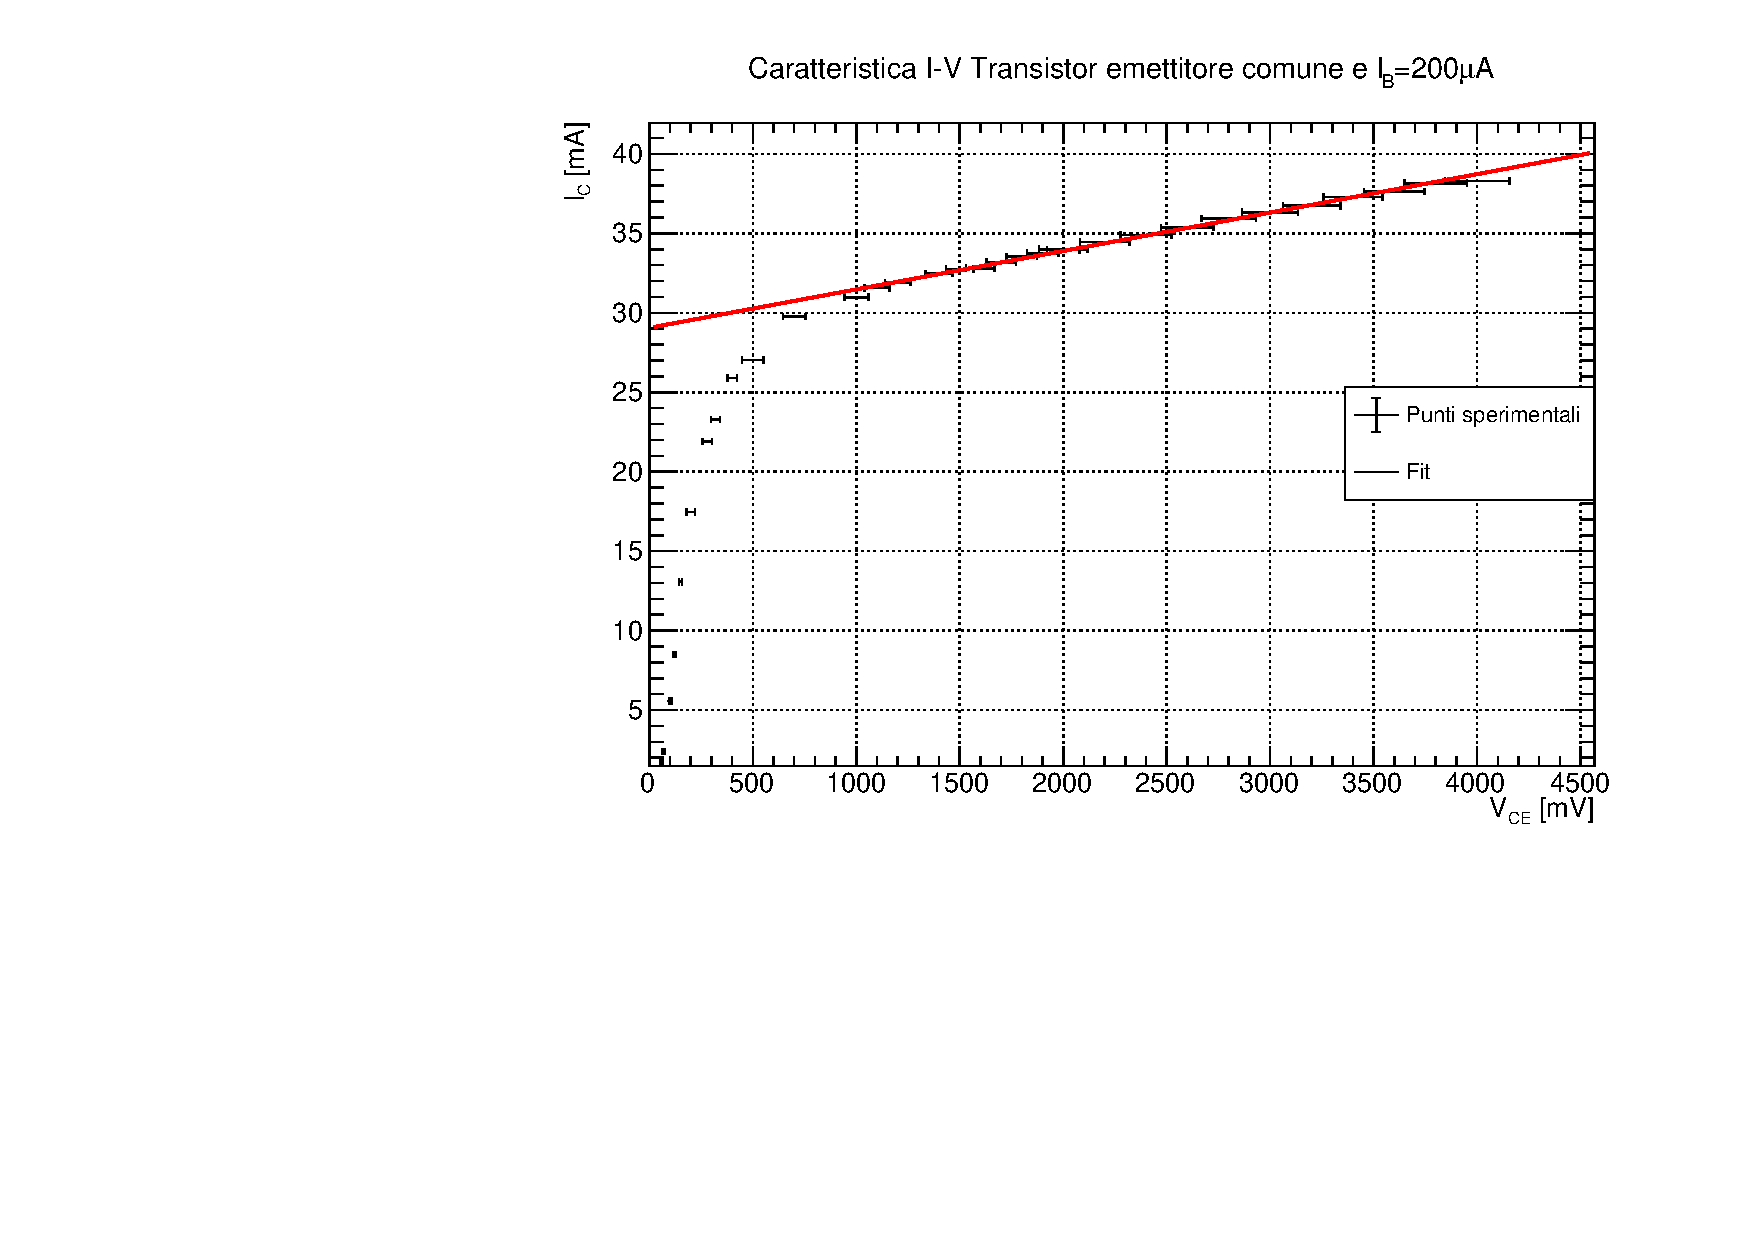
\includegraphics[width=0.9\linewidth]{../200 muA/c1}
	\caption{Caratteristiche in uscita del transistor con corrente di base a -200 $ \mu A $}
	\label{fig:corrente 200}
\end{figure}
\subsection{Corrente a $ -100\,\mu A $}
Dal fit dei dati in tabella (\ref{tab:100muA}), riportato nel grafico in figura \ref{fig:corrente 100}, abbiamo ottenuto come tensione di Early $ V_{A}=-16130\pm510\ mV $, mentre la resistenza in uscita è risultata $ \frac{\Delta V_{CE}}{\Delta I _{C}}=985\pm28\ \Omega$. Per il suo inverso, ovvero la conduttanza, abbiamo ottenuto $ g=(101.5\pm2.9)\cdot 10^{-5} A/V $. Si può chiaramente vedere sia l'andamento lineare, con inclinazione dovuto all'effetto Early, che il gomito della curva quando la corrente inizia a variare esponenzialmente.
	\begin{figure}[H]
		\centering
		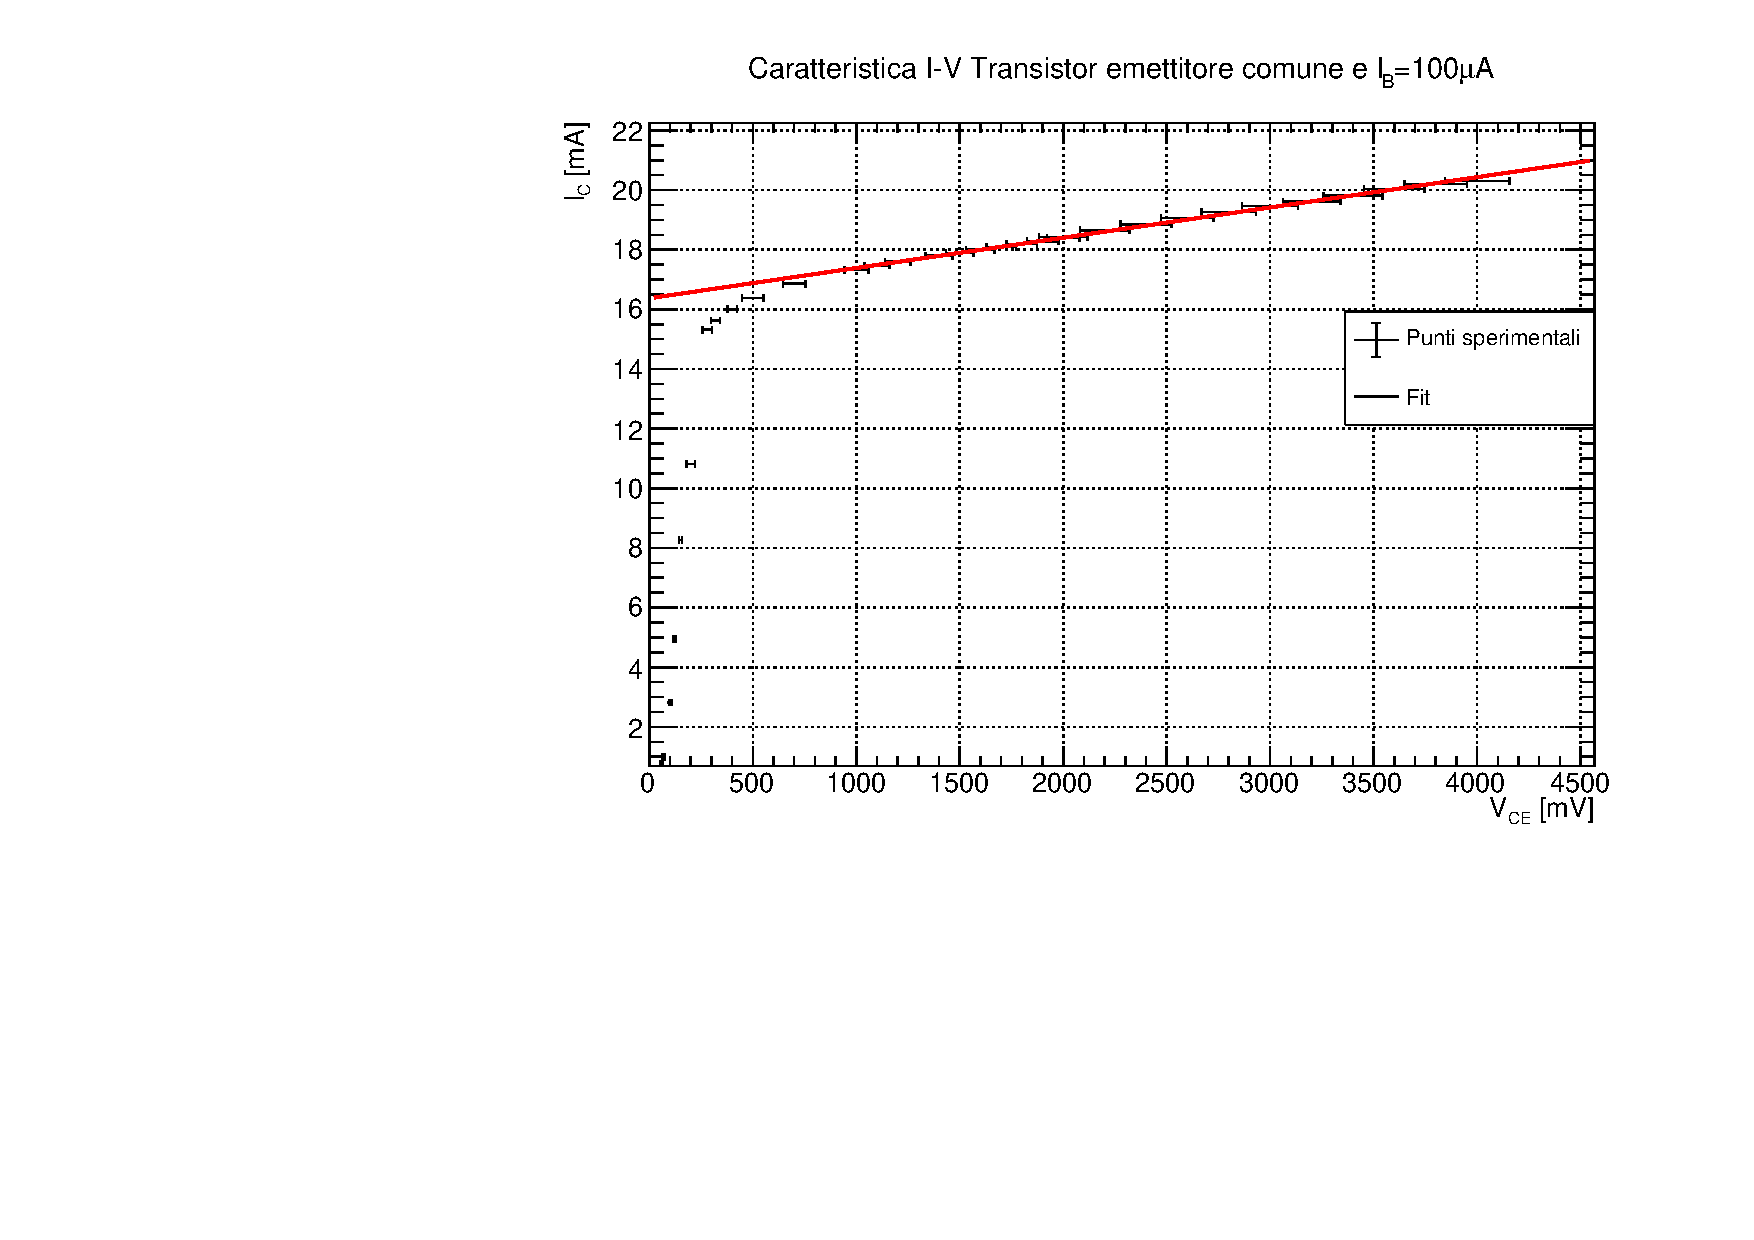
\includegraphics[width=0.9\linewidth]{../100 muA/c1}
		\caption{Caratteristiche in uscita del transistor con corrente di base a -100 $ \mu A $}
		\label{fig:corrente 100}
	\end{figure}
\subsection{Multigrafo con entrambe le curve}
Di seguito è riportato in figura il multigrafo (\ref{fig:multigrafo}) contenente entrambe le curve. Da quest'ultimo abbiamo ricavato una stima del guadagno di corrente misurando per ogni valore di tensione preso la differenza di corrente tra i punti e diviso per la differenza delle correnti di base secondo la formula:
\begin{equation}
	\beta=\frac{\Delta I_{C}}{\Delta I_{B}}
\end{equation}
	\begin{figure}[H]
		\centering
		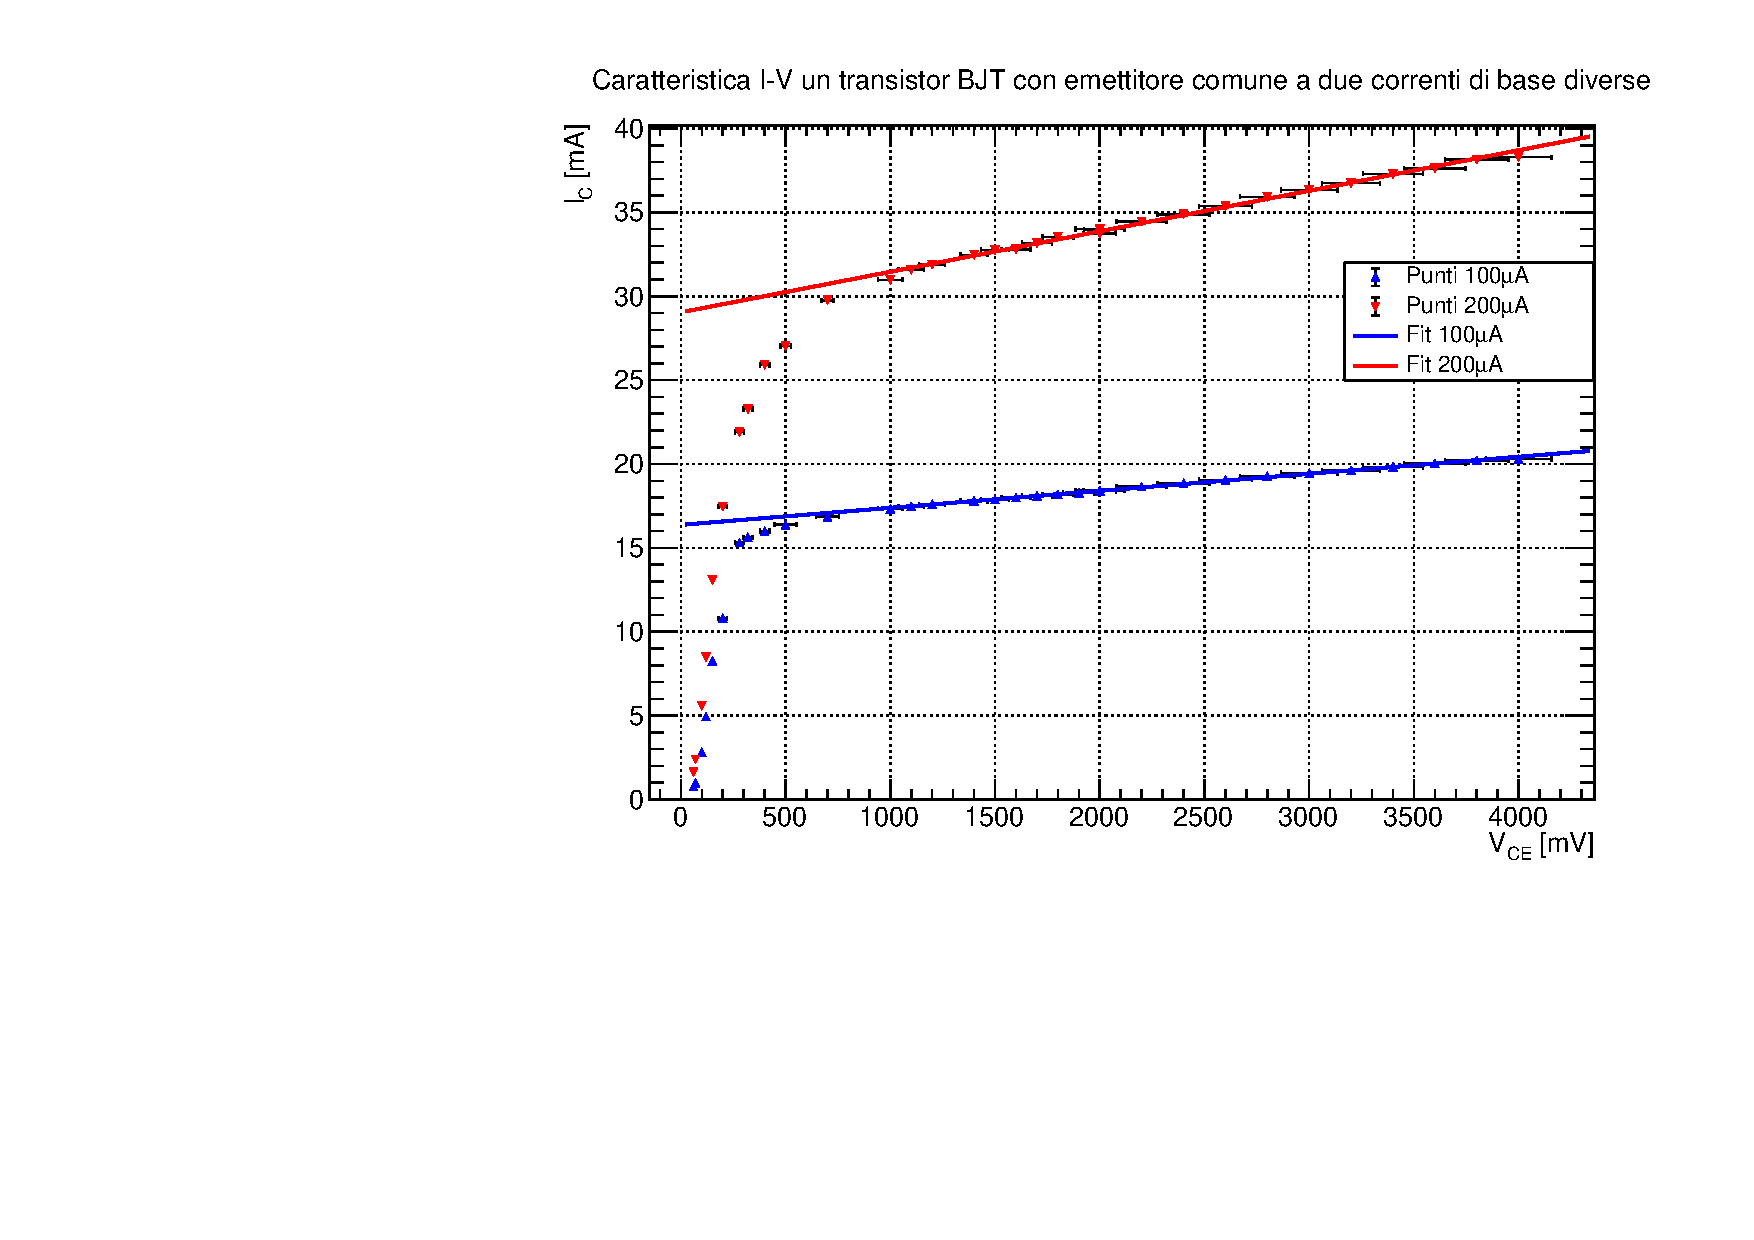
\includegraphics[width=0.9\linewidth]{../c1}
		\caption{Caratteristiche in uscita del transistor. In rosso per la corrente di base a -200 $ \mu A $ e in blu per la corrente di base a -100 $ \mu A $}
		\label{fig:multigrafo}
	\end{figure}
Da una media di 20 misure prese nella zona con andamento lineare abbiamo ottenuto $ \beta =159\pm 13 $, dove per l'errore abbiamo usato la deviazione standard.
\section*{Conclusioni}
Le misure delle caratteristiche in uscita del transistor si sono rivelate qualitativamente in accordo con la teoria riproducendo l'andamento prima lineare nella regione attiva e poi esponenziale in quella di saturazione. Evidente è l'inclinazione delle due rette dovuto all'effetto Early, il cui valore di tensione è risultato in entrambe le curve dell'ordine di grandezza previsto.  
Anche il parametro b, ovvero la resistenza in uscita, e di conseguenza il suo inverso g sono risultati dell'ordine di grandezza aspettato per entrambe le due curve. 
Infine, il valore stimato di $ \beta $ è risultato anch'esso compatibile con i valori di aspettazione.
Fa cagare come conclusione ma non c'ho sbatti. Evviva Kirby
\newpage
\begin{figure}
	\centering
	\includegraphics[width=0.9\linewidth]{../kirby}
\end{figure}
\end{document}
